%%%%%%%%%%%%%%%%%%%%%%%%
%
%   Thesis template by Youssif Al-Nashif
%
%   May 2020
%
%%%%%%%%%%%%%%%%%%%%%%%%

\chapter{Literature Review}
\label{literature-review}


%---- Introduction



\indent Previous research work in Learning Analytics (LA) involve everything from surveys of machine learning techniques in developing education platforms, to novel 
statistical methods in data-driven education. Methods typically form solutions from predictive models estimating student performance on examinations and clustering models 
between students and questions \cite{barbu_data_nodate}. Some applications of these methods incorporate user modeling, identifying professors, students, and other faculty in 
relation to coursework and how those researchers engage with online systems to provide insight to analytical platforms. LA typically focuses on the educational challenge while 
Educational Data Mining (EDM) focuses on developing algorithms and/or models \cite{hilliger_evaluating_2019}.

\indent Most applications make use of publicly available datasets \shortcites{romero_educational_2020} or data obtained from the relevant research university in which the 
study takes place. This enables peer review and rapid iteration of numerous machine learning and analytical concepts across different universities \cite{barbu_data_nodate}
\cite{romero_educational_2020}\cite{hilliger_evaluating_2019}.  Specific data about users is typically obtained when the course in question is fully online or a Massively 
Open Online Course (MOOC). Work in this field has culminated in massive open source projects and publicly available work such as MIT’s Mapping Lab and even student-driven 
applications like MIT Crosslinks. In these endeavors, MIT makes use of network modeling,  factor analysis, and machine learning techniques to 
create a robust ecosystem of tools to aid education at the institution \cite{willcox_network_2017}. 

Dimensionality reduction methods like Multi-Dimensional Scaling (MDS) \cite{jjs} and Correspondence Analysis are used to generate latent space representations of the dynamics 
present in text data by utilizing distance metrics and the Singular Value Decomposition (SVD) respectively.  MDS allows for dynamic exploration of different distance metrics 
for use with text data, some of which are highly robust to features of text data.  Correspondence Analysis uses SVD to get latent space representations of text data,  where 
the new corresponding dimensions decrease successively in proportion of variance explained. 

\indent Novel methods like Sparse Factor analysis, introduced by A.S. Lan, et al. enhance previous work done in the field of LA, enabling question-concept association graphs 
to be generated. Different from the approach discussed in this proposal, question-concept associations allow a bank of questions to be linked by overarching concepts pertaining 
to a number of different courses, aligning students with possible avenues to make up shortcomings from missing fundamental concepts \cite{lan_sparse_nodate}
\cite{willcox_network_2017}. Sparse Factor analysis takes the approach of a normal factor analysis, abstracting conceptual knowledge of learners and constructing 
association graphs, giving insight to their relationships. In the sparse case however, each question measures the learner’s knowledge on only a few concepts, resulting in a 
sparse questions-concept association matrix.  See Figure \ref{fig:sparfa}. This approach, while originally applied to the question-concept association level, is also applicable 
to the course-concept association level discussed here. 




\begin{figure}[ht]
\centering

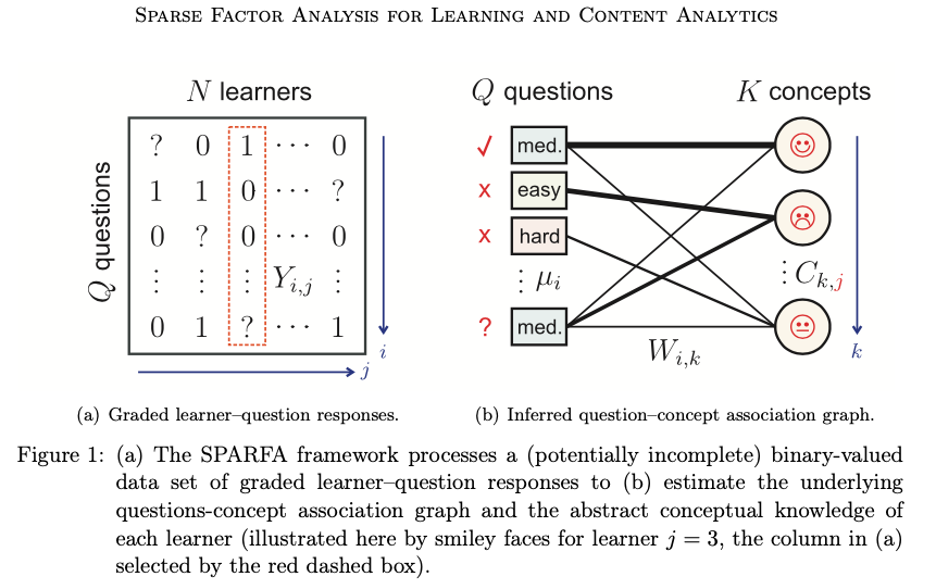
\includegraphics[width = \textwidth]{Content/images/sparfa.png}
\caption{Sparse Factor Analysis applied at the questions-concept association level but applicable to the more macro course-concept association level}
\label{fig:sparfa}
\end{figure}




%%%%%%%%%%






